%\documentclass[aps,prd,nofootinbib]{revtex4-1}
\documentclass[singlepage,notitlepage,nofootinbib,11pt]{revtex4-1}
\usepackage{amsmath}
\usepackage{amssymb}
\usepackage{graphicx}
\usepackage{subfig}
\usepackage{epsfig}
\usepackage{listings}
\usepackage[hidelinks,hyperfootnotes=false,bookmarks=false,colorlinks=true]{hyperref}

\newcommand{\eq}[1]{\begin{align*}#1\end{align*}}
\newcommand{\pmat}[1]{\begin{pmatrix}#1\end{pmatrix}}
\newcommand{\center}[1]{\begin{center}#1\end{center}}
\def\<{\langle}
\def\>{\rangle}
\def\l{\left}
\def\r{\right}

\begin{document}
\title{Problem Set 5 - G6080}
\author{Victor Genty}
\email{vgenty@nevis.columbia.edu}
\homepage{www.nevis.columbia.edu/~vgenty}
\date{\today}
\begin{abstract}
\centering
Source code can be found at \href{https://github.com/vgenty/G6080/tree/master/final}{github.com/vgenty/G6080/final}
\end{abstract}
\maketitle
\section*{Introduction}
Blah
\section*{1.1 Setup}
\begin{enumerate}
\item Te updating scheme in Eq. (2) is unitary because it preserves the integral squared norm of the state vector in time i.e.
  \begin{align*}
    \int_{\mathbb{R}} dx \left|\phi(t+\Delta t)\right|^2 = \int_{\mathbb{R}} dx \left|\phi(t)\right|^2.
  \end{align*}
  Therefore it's sufficient to check if the updating scheme is norm preserving at $n+1$ and $n$. So,
  \begin{align*}
    \left|\phi^{(n+1)}\right|^2 &= \left|\frac{1-i H \Delta t/2}{1+i H \Delta t/2}\right|\left|\phi^{n}\right|^2 \\
    &= \frac{1-i H \Delta t/2}{1+i H \Delta t/2}\cdot\frac{1+i H^{\dagger} \Delta t/2}{1-i H^{\dagger} \Delta t/2}.
  \end{align*}
  Now the Hamiltonian is hermitian, $H = H^{\dagger}$ so,
  \begin{align*}
    \frac{1-i H \Delta t/2}{1+i H \Delta t/2}\cdot\frac{1+i H \Delta t/2}{1-i H \Delta t/2} &=  1,\\
  \end{align*}
  as the numerator and denominator cancel leaving,
  \begin{align*}
    \left|\phi^{n+1}\right|^2 = \left|\phi^n\right|^2.
  \end{align*}
  Therefore the updaing scheme is unitary.
\item The Schrodinger equation and be nondimensionalized with the substitutions,
  \begin{align*}
    \widetilde{\phi}&=\phi\sqrt{\frac{\hbar}{m c}}\\
    \widetilde{x}&=x\left(\frac{mc}{\hbar\right)}\\
    \widetilde{t}&=t\left(\frac{mc^2}{\hbar}\right)\\
    \widetilde{V}&=V\left(\frac{1}{mc^2}\right),
  \end{align*}
  leaving the Schrodinger equation as,
  \begin{align*}
    -\frac{1}{2}\frac{\partial^2}{\partial\widetilde{x}^2}\widetilde{\phi}+\widetilde{V}\widetilde{\phi} = i \frac{\partial}{\partial\widetilde{t}}\widetilde{\psi}.
  \end{align*}
  This gives the updating scheme the following form,
  \eq{
    \chi_{j+1}^{(n)}+\left(-2+\frac{4i\widetilde{\epsilon}^2}{\Delta\widetilde{t}}-2\widetilde{\epsilon}^2\widetilde{V_j}\right)\chi_j^{(n)} + \chi_{j-1}^{(n)} = \frac{8i\widetilde{\epsilon}^2}{\Delta\widetilde{t}}\phi_j^{(n)}.
  }
  The total range of the simulation is fixed to $-1 < x < 1$. We also set the mass $m$ equal to 1. {\bf come back to me}
\end{enumerate}
\section*{1.2 Evolution of a wavepacket}
We start with a normalized gaussian wave packet at $t=0$,
\eq{
\phi(x,t=0) = \frac{1}{\sqrt{\sigma \sqrt{\pi}}}\exp\left(ikx\right)\exp\left(-(x-x_0)^2/\left(2\sigma^2\right)\right).
}
This particular wave packet has a fixed expecation energy value given by,
\begin{align*}
  \<E\> &= \<\phi|E|\phi\> = \<\phi|\frac{p^2}{2m}|\phi\> = \int_{\mathbb{R}}dx\<\phi|x\>-\frac{\hbar^2}{2m}\frac{\partial^2}{\partial x^2}\<x|\phi\> \\
  &= \frac{p^2}{2m} + \frac{\hbar^2}{2 m \sigma^2},
\end{align*}
and with our choice of units is
\eq{
\<E\> = \frac{k^2}{2} +  \frac{1}{4\sigma^2}.
}
Rearranging we can choose the input momentum based on the given energy,
\eq{
k = \sqrt{2 E - \frac{1}{2\sigma^2}}
  }
I checked my implementation of the algorithm, specifically my implementation of the LU factorization of the tridiagonal matrix. I evolved the free particle for a total time step of 1000, 500 steps in the forward direction then fliping the sign of the time step $dt$ and then evolving 499 steps in the reverse direction to check for unitarity. Snapshots of the wavepackets are shown in Fig. \ref{evolution}. The wavepackets are nearly identical before and after the evolution. As the gaussian propogates it spreads out in position as epected from a free particle. The elongated wave at $t=T/2$ then begins narrowing as the algorithm is reversed. We check the unitarity of the state as a function of time and plot in Fig. \ref{unitarity}. The unitarity of the state does not deviate from one out of IEEE double precision during the duration of the test simulation indicating fantastic conserved unitarity.
\begin{figure}[h]
  \centering
  \captionsetup[subfigure]{labelformat=empty}
  \subfloat[][]{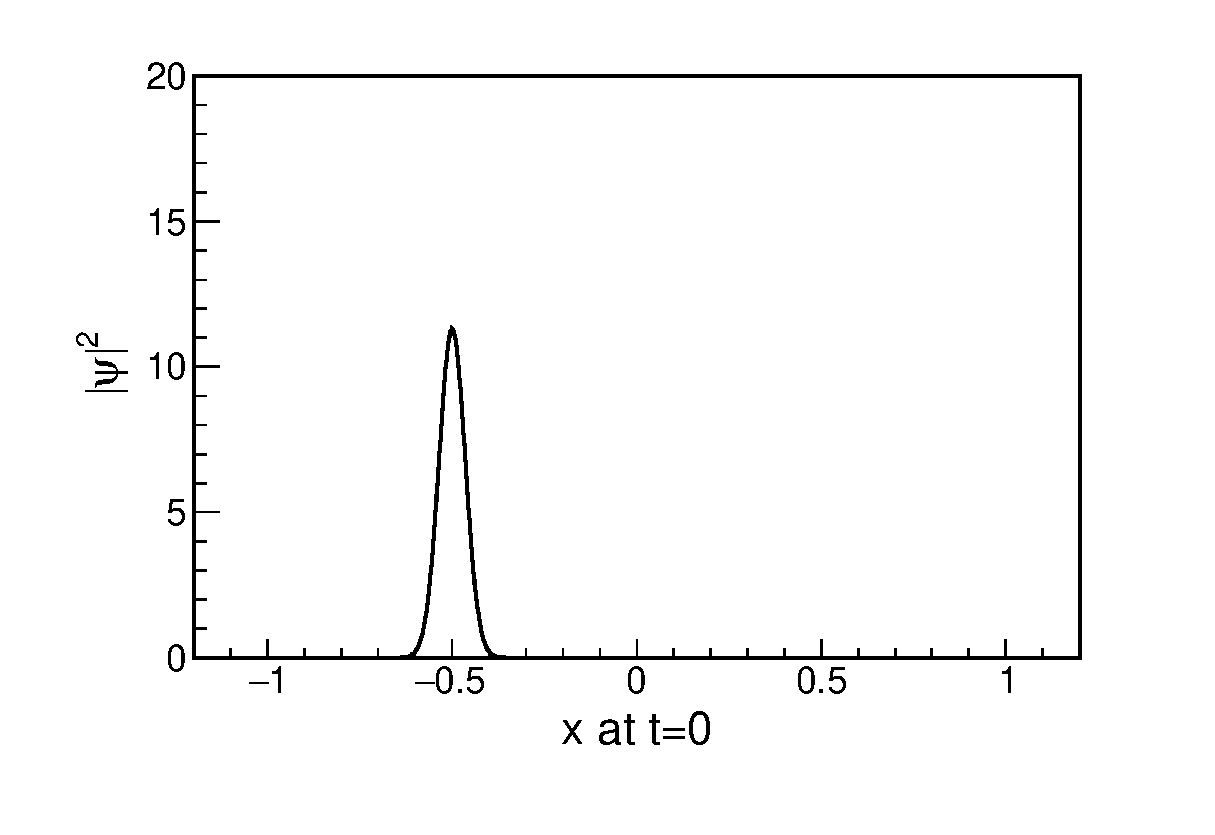
\includegraphics[width=0.5\textwidth]{figures/packet_t0.eps}}
  \subfloat[][]{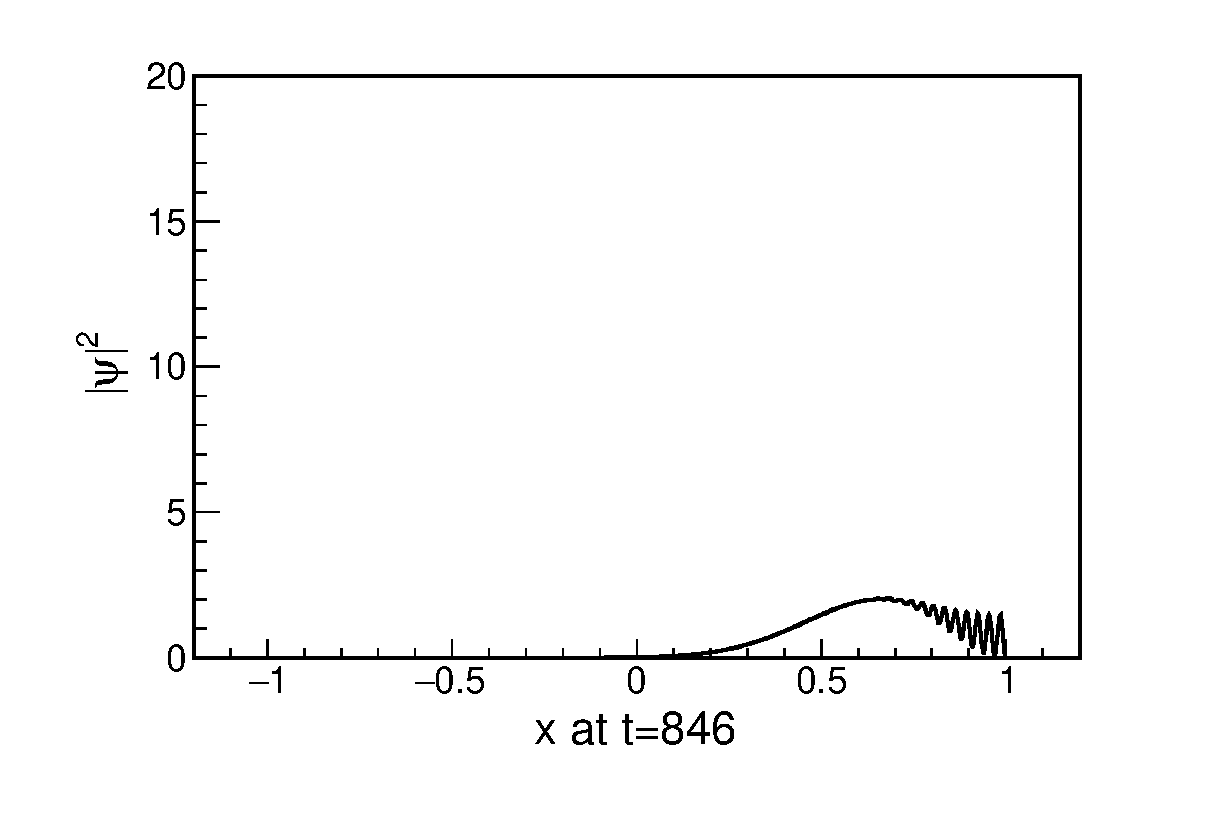
\includegraphics[width=0.5\textwidth]{figures/packet_t846.eps}}\\
  \subfloat[][]{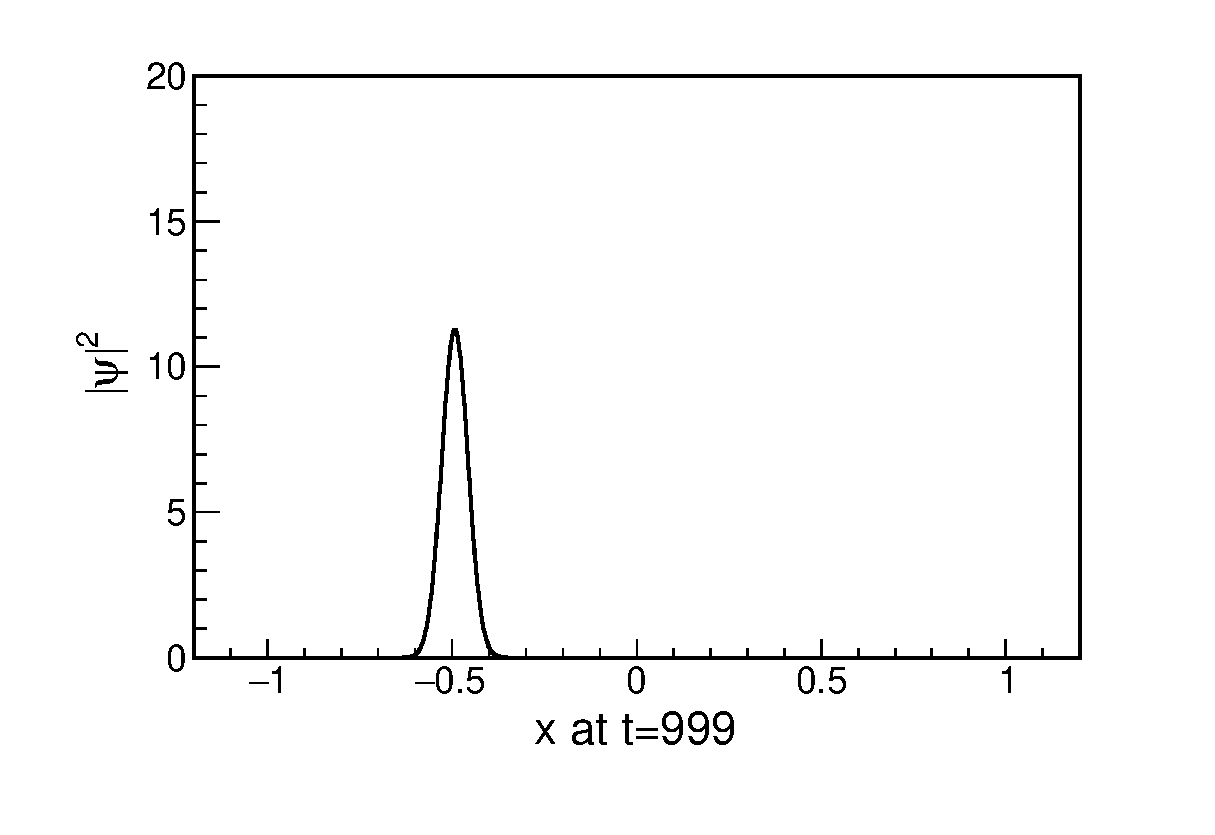
\includegraphics[width=0.5\textwidth]{figures/packet_t999.eps}}
  \caption{\label{evolution} Position space snap-shots of the specified gaussian wavepacket at three different time slices. The top left pane shows the initial state at $t=0$. The top right pane shows the impact of the gaussian wave packet with the infinite wall in reversed time. The bottom pane shows the state returning to its initial configuration.}
\end{figure}
\begin{figure}[h]
  \centering
  \captionsetup[subfigure]{labelformat=empty}
  \subfloat[][]{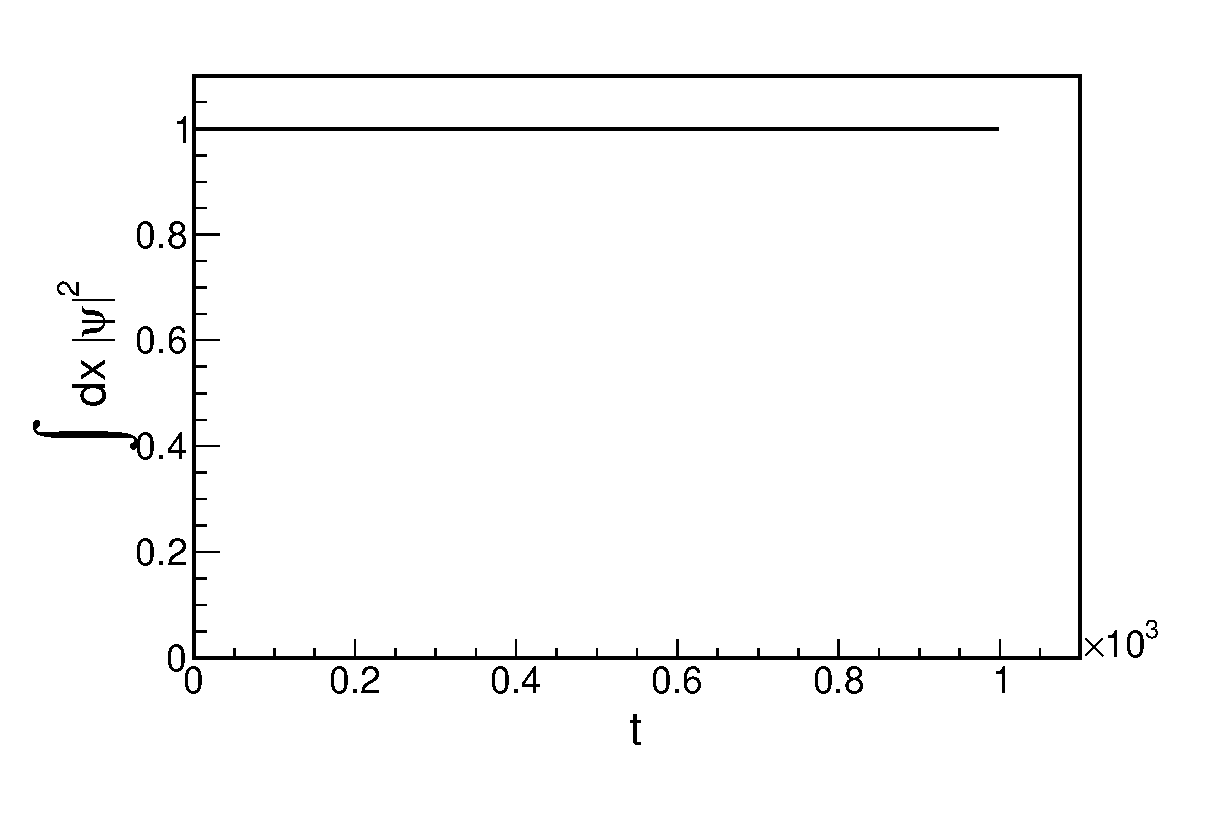
\includegraphics[width=0.5\textwidth]{figures/unitarity.eps}}
  \caption{\label{unitarity} Integral norm squared of gaussian wave packet as a function of time. }
\end{figure}
\subsection*{1.3 Scattering from a step function potential}
We scatter wavepackets of varying widths and incident energies at step potentials. For this problem we must ensure the wavepacket is sufficiently localized and therefore energetic enough to quickly scatter off the step potential without encountering effects from hitting the infinite walls.
\end{document}
